\section{Metodologia}
\label{sec:metodologia}

Para o cumprimento dos objetivos gerais e específicos do trabalho foram considerados catorze requisitos -- dez funcionais e quatro desejáveis -- pré-estabelecidos por um cliente fictício. Os requisitos estão listados abaixo:
\vspace{1 mm}

\textbf{Funcionais}
\begin{enumerate}
	\item Ser capaz de estabelecer comunicação com operador na superfície.
	\item Ser capaz de submergir e emergir de forma controlada.
	\item Ser capaz de se locomover em baixo d'água com uma velocidade de 2 m/s.
	\item Ser capaz de seguir trajetória pré-estabelecida.
	\item Ser capaz de mapear o leito submarino abaixo (angulação mínima de $ \pm $ 10°).
	\item Ser capaz de localizar no mapa um objeto pré-definido.
	\item Ser capaz de se deslocar até uma coordenada (3D) ou objeto pré-definido.
	\item Ser capaz de detectar ``sinal de socorro'' e se deslocar até a fonte emissora.
	\item Ser capaz de transmitir dados, inclusive a localização (3D) em tempo real.
	\item Ser capaz de armazenar o caminho percorrido para o cumprimento da missão.
\end{enumerate}

\textbf{Desejáveis}

\begin{enumerate}[resume]
	\item O protótipo deve suportar pressões correspondentes a pelo menos 10 mca.
	\item O protótipo deve ser ``bem montado'' e ``apresentável''.
	\item Deve-se preservar aspectos de segurança na operação, resgate e manutenção.
	\item Deve-se desenvolver IHM para monitoramento em tempo real.	
\end{enumerate}

\vspace{1 mm}

A metodologia adotada para levantamento de ideias, ponderação de requisitos e seleção preliminar de componentes está descrita na Figura \ref{fig:metodologia}. As subseções a seguir detalham o que foi desenvolvido em cada etapa da metodologia.

\begin{figure}[h]
	\centering
	\caption{Metodologia adotada para o projeto}
	\label{fig:metodologia}
	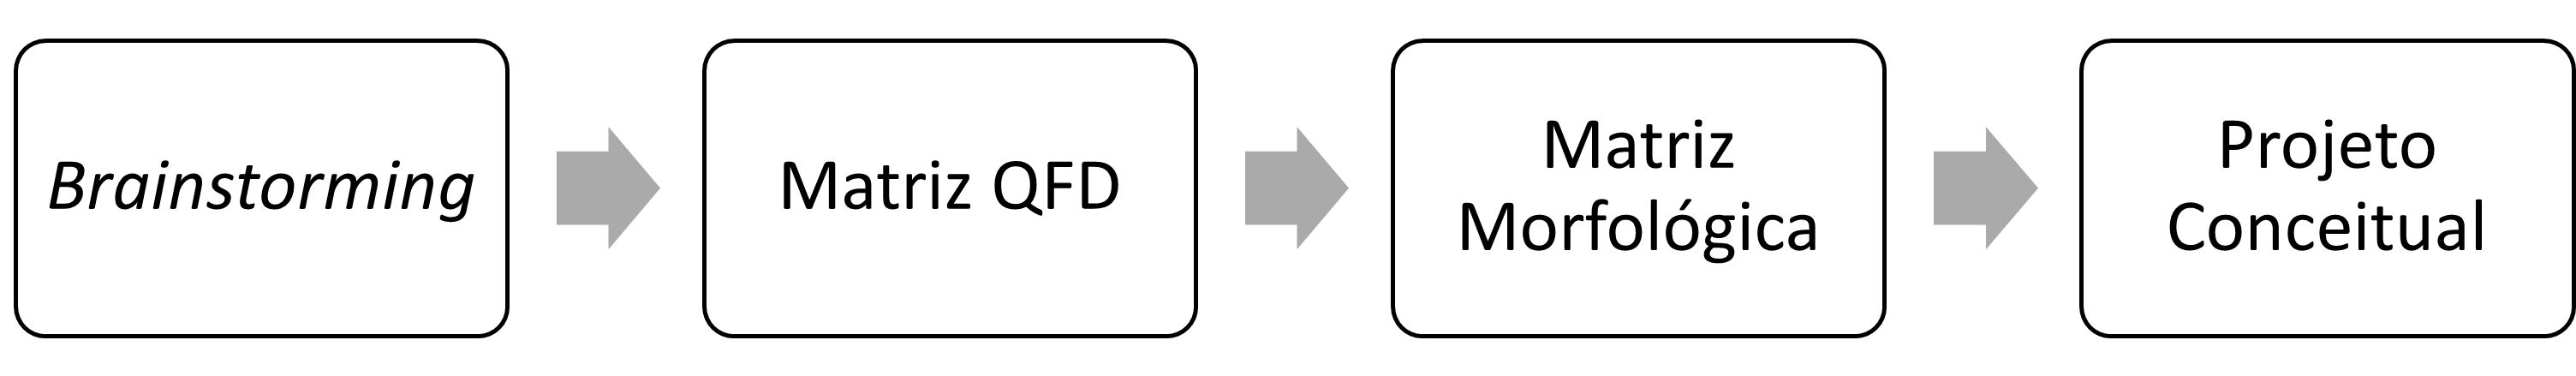
\includegraphics[width=0.7\linewidth]{images/metodologia}\\
	\footnotesize Fonte: Autores
\end{figure}

\subsection{\textit{Brainstorming}}
\label{subsec:brainstorming}

Na fase de \textit{brainstorming} foram levantadas algumas soluções que poderiam atender ao maior número possível de requisitos. Ao término dessa etapa, a equipe chegou a um conceito inicial, que está mostrado na Figura \ref{fig:conceito-inicial}.

\begin{figure}[h]
	\centering
	\caption{Conceito inicial da solução}
	\label{fig:conceito-inicial}
	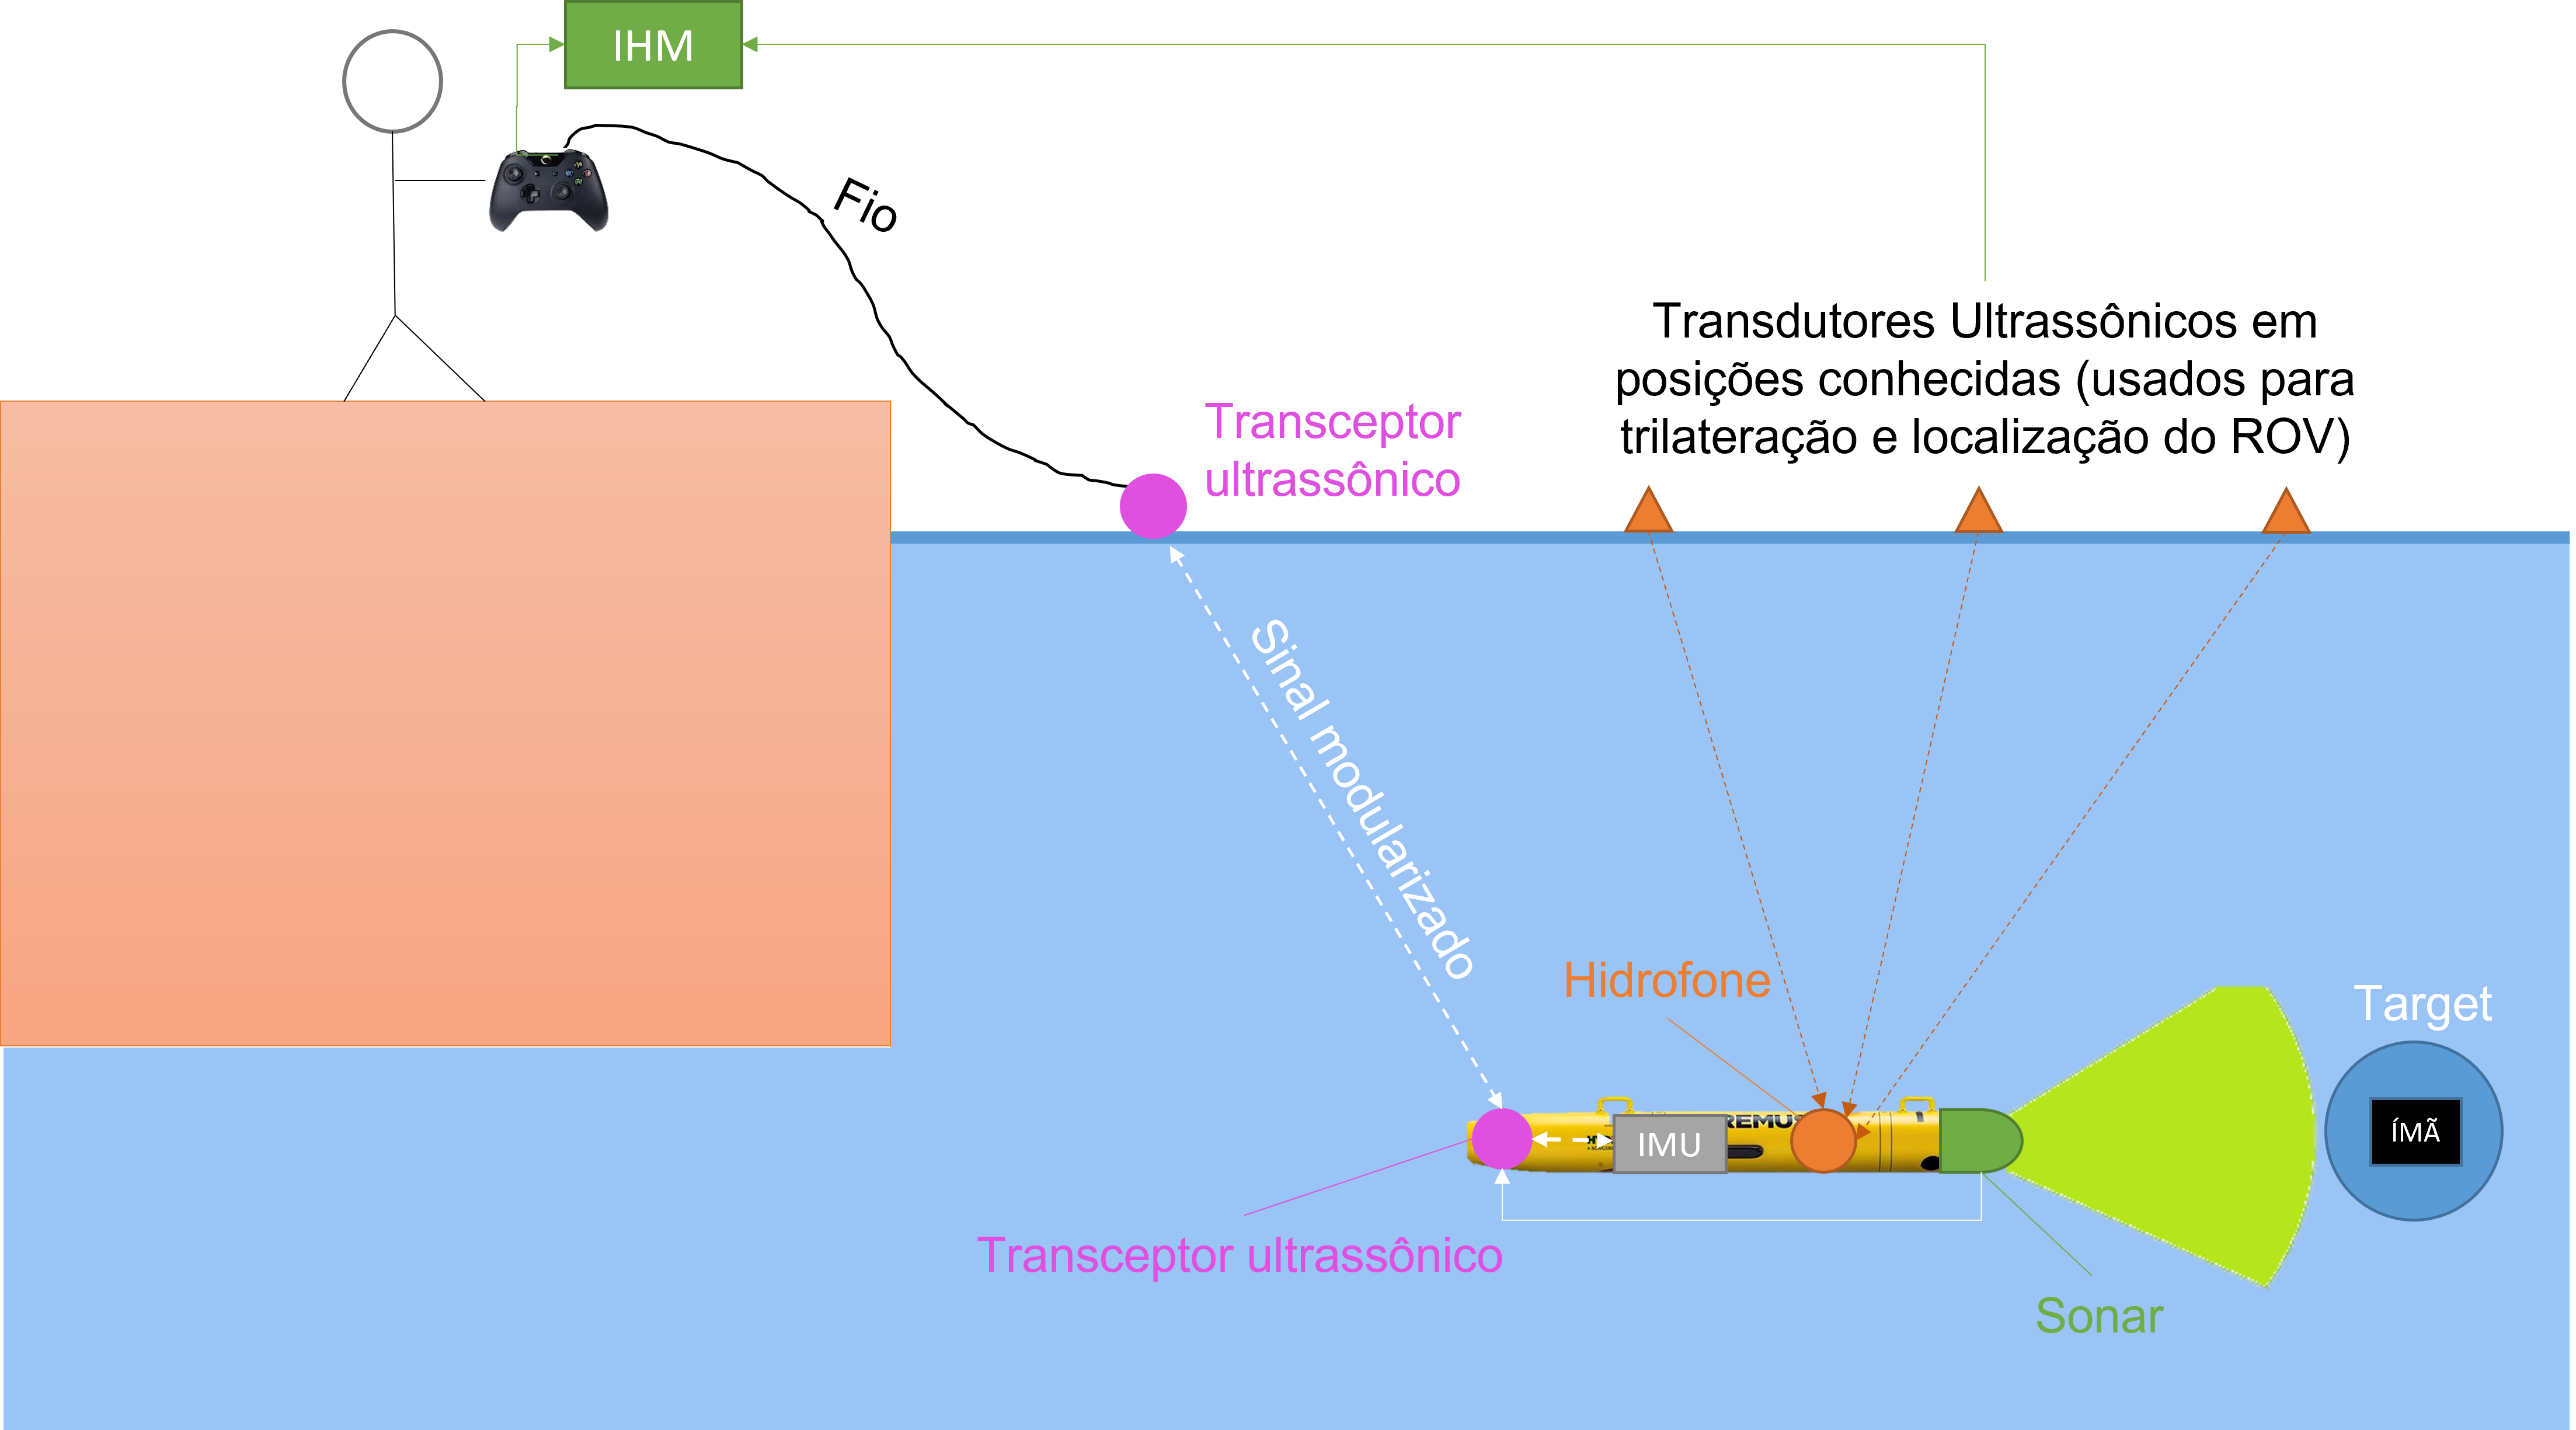
\includegraphics[width=1\linewidth]{images/conceito-inicial}\\
	\footnotesize Fonte: Autores
\end{figure}

Nesse conceito, o operador seria responsável por enviar comandos de deslocamento para um transceptor ultrassônico -- que estaria dentro de uma bóia na superfície -- através de um controle. O comando seria então convertido em um sinal modularizado para ser enviado ao transceptor ultrassônico presente no ROV. Em seguida, esse sinal seria decodificado e o ROV se deslocaria para a posição desejada. 

A localização do ROV seria periodicamente monitorada por três transdutores ultrassônicos presentes na superfície da água, que atuariam como \textit{ground-truth}, recebendo a informação de um hidrofone presente no ROV e calculando a localização por meio de trilateração. Essa informação seria então enviada para a inteface homem-máquina (IHM) via cabo ou RF.

A medida em que o ROV se aproximasse do objeto de interesse -- que estaria emitindo sinal acústico --, haveria uma amplificação do sinal do sonar embarcado, que seria transmitido para o transceptor ultrassônico presente no ROV e enviado de volta para o operador. O objeto teria também um ímã para facilitar a captura e resgate.

O mapeamento do leito seria feito de modo \textit{offline} por outro sensores ultrassônicos embarcados no ROV. O registro da trajetória também não seria feito em tempo real, mas de modo \textit{offline} por meio do rastro calculado pela IMU (do inglês \textit{Inertial Measurement Unit}).


\subsection{Matriz QFD}
\label{subsec:matriz-qfd}

Após obtenção de um conceito inicial, a equipe utilizou a Matriz QFD (do inglês \textit{Quality Function Deployment}) para conversão das necessidades do cliente fictício em requisitos factíveis de projeto. Nessa etapa foram avaliadas as relações entre as necessidades e os requisitos, assim como as correlações dos requisitos entre si. Não foi feita uma análise de concorrentes. Ao término do preenchimento da QFD, cujo recorte está mostrado na Tabela \ref{tab:qfd-brov-recorte}, foi possível determinar a ordem de priorização dos requisitos. Os principais requisitos listados foram:

\begin{enumerate}
	\item Comunicação \textit{wireless}.
	\item Localizar ROV.
	\item Seguir trajetória pré-estabelecida.
\end{enumerate}

\begin{table}[h!]
	\centering
	\caption{Matriz QFD}
	\label{tab:qfd-brov-recorte}
	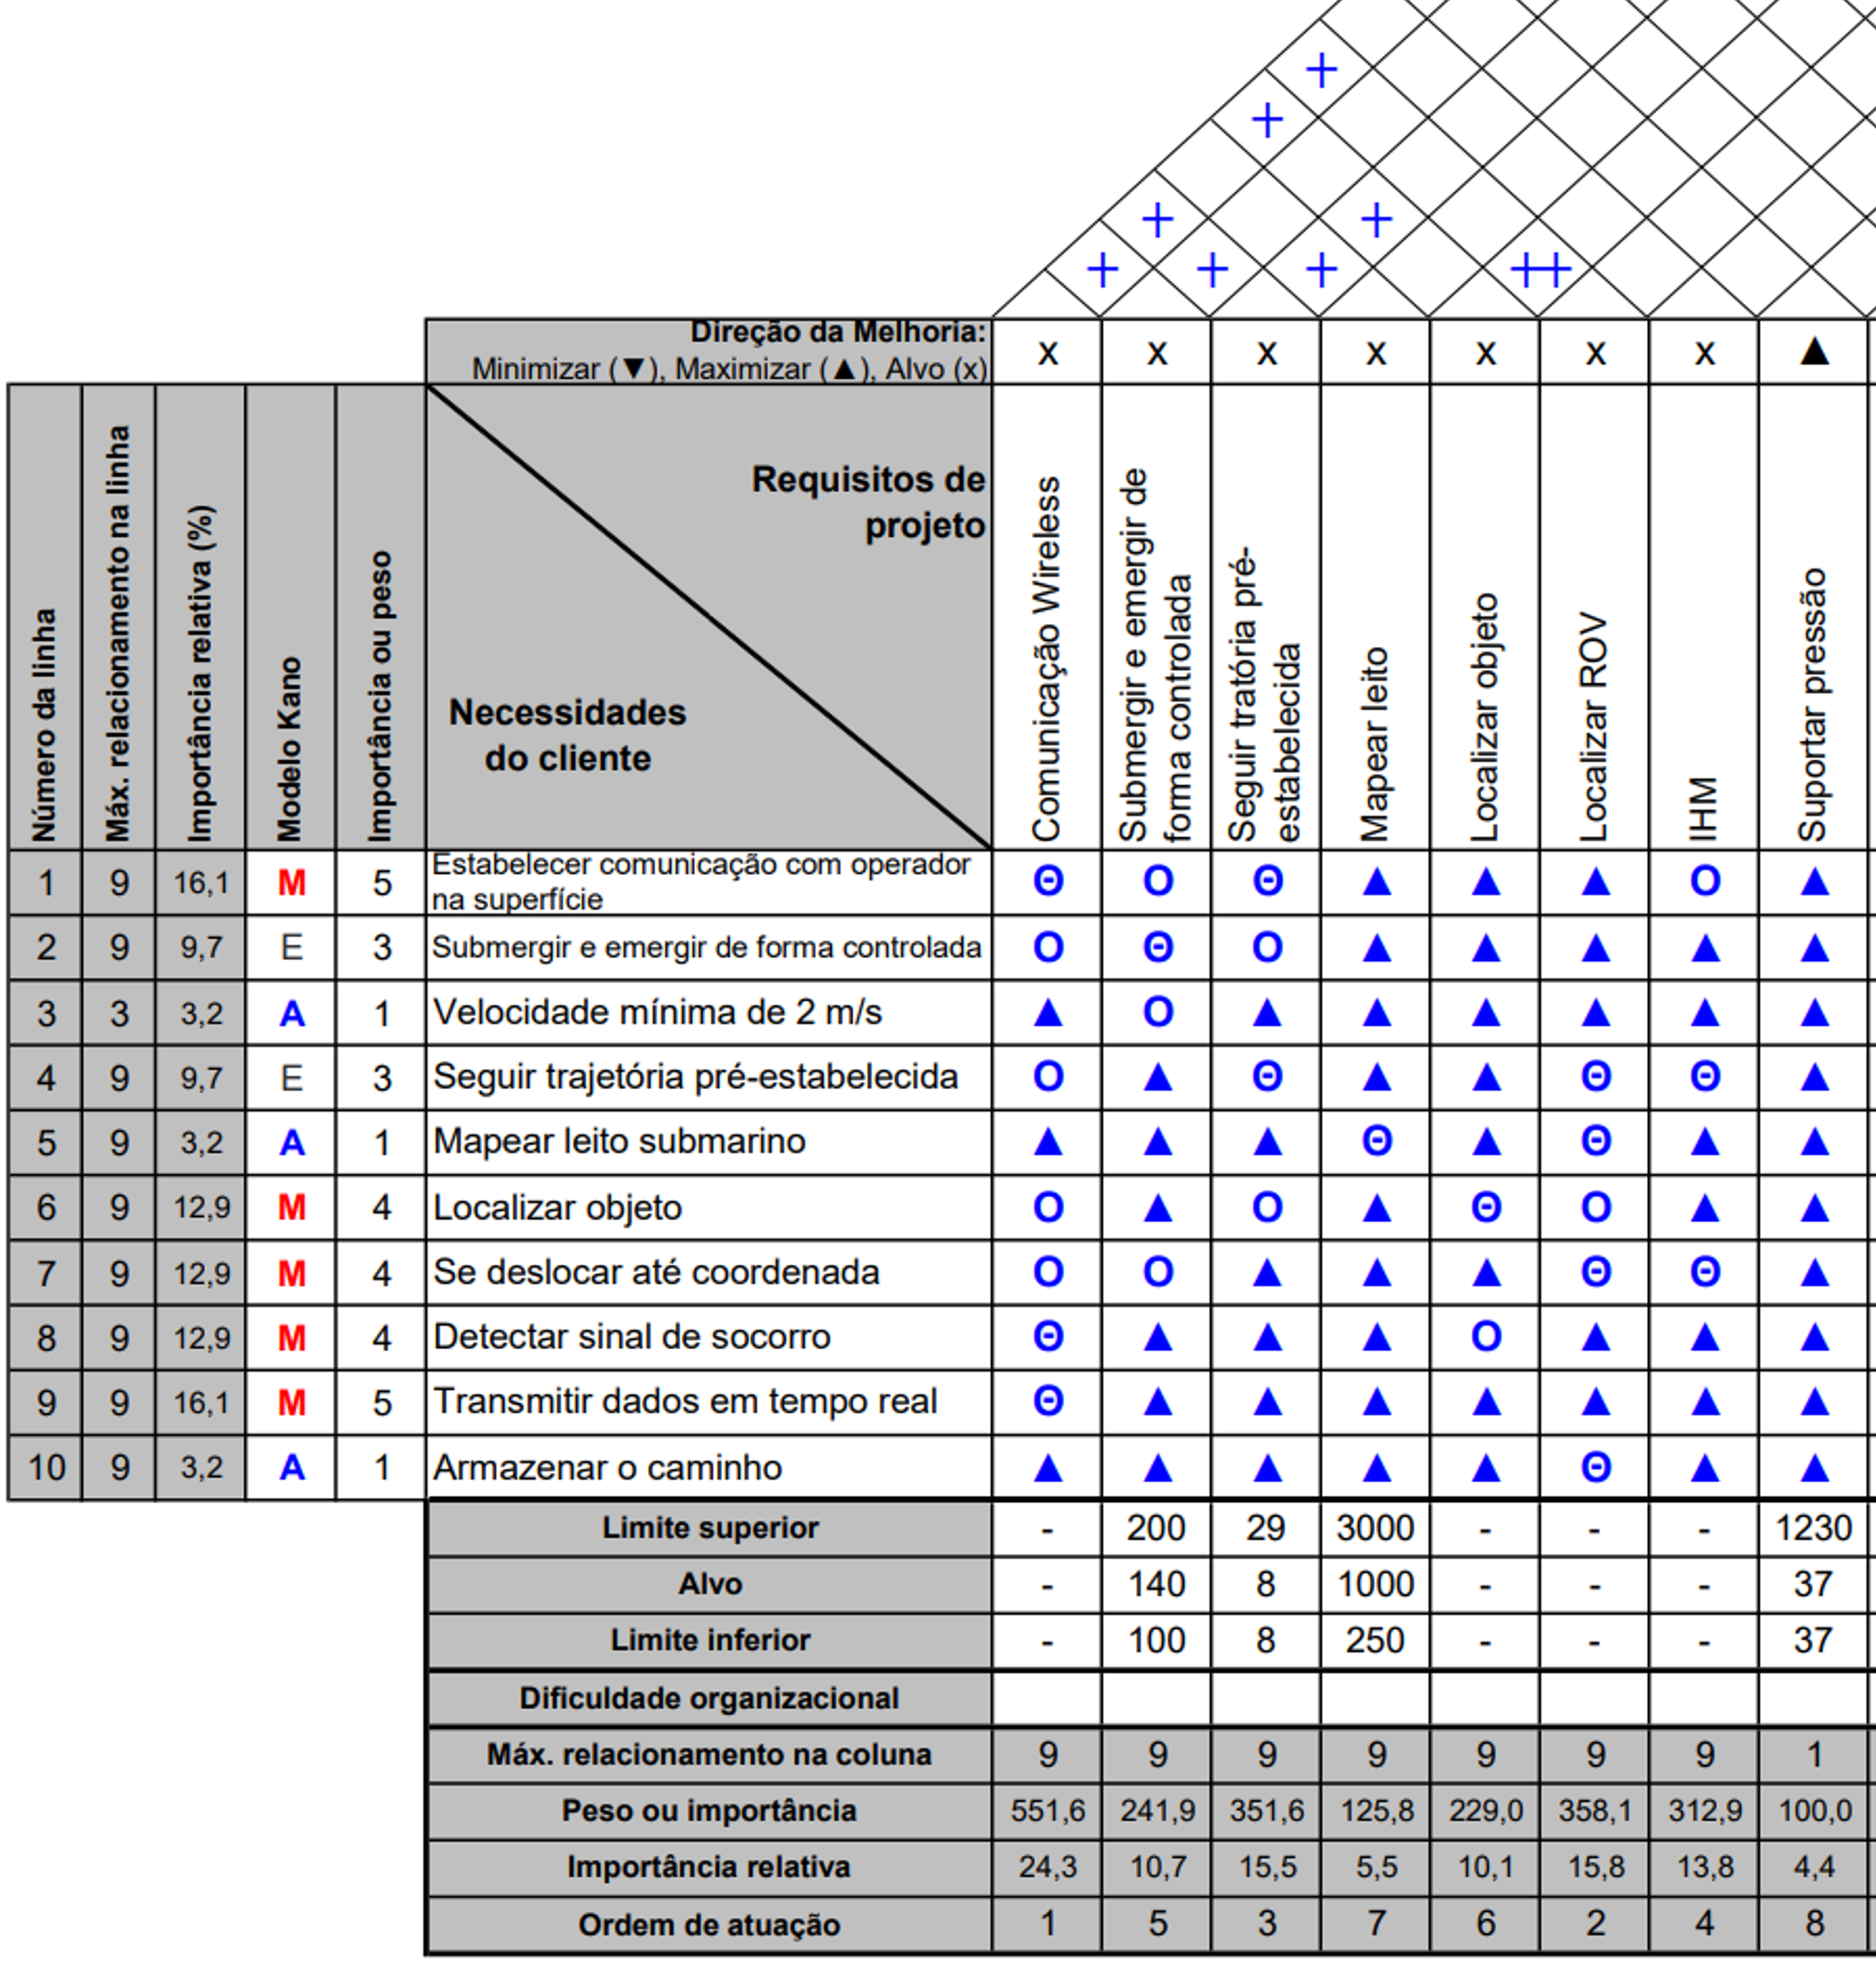
\includegraphics[width=1\linewidth]{images/QFD-BROV.png}\\
	\footnotesize Fonte: Autores
\end{table}

\subsection{Matriz Morfológica}
\label{subsec:matriz-morfologica}

A matriz morfológica, mostrada na Tabela \ref{tab:matriz-morfologica}, foi utilizada para seleção preliminar dos componentes e sistemas que viriam compor o ROV, de modo a solucionar cada requisito de projeto. Ao término do preenchimento da matriz morfológica, o conceito inicial sofreu alterações, como substituição e inclusão de novos sensores. 
%Os argumentos para seleção de alguns dos componentes estão expostos a seguir.

\begin{table}[h!]
	\centering
	\caption{Matriz morfológica}
	\label{tab:matriz-morfologica}
	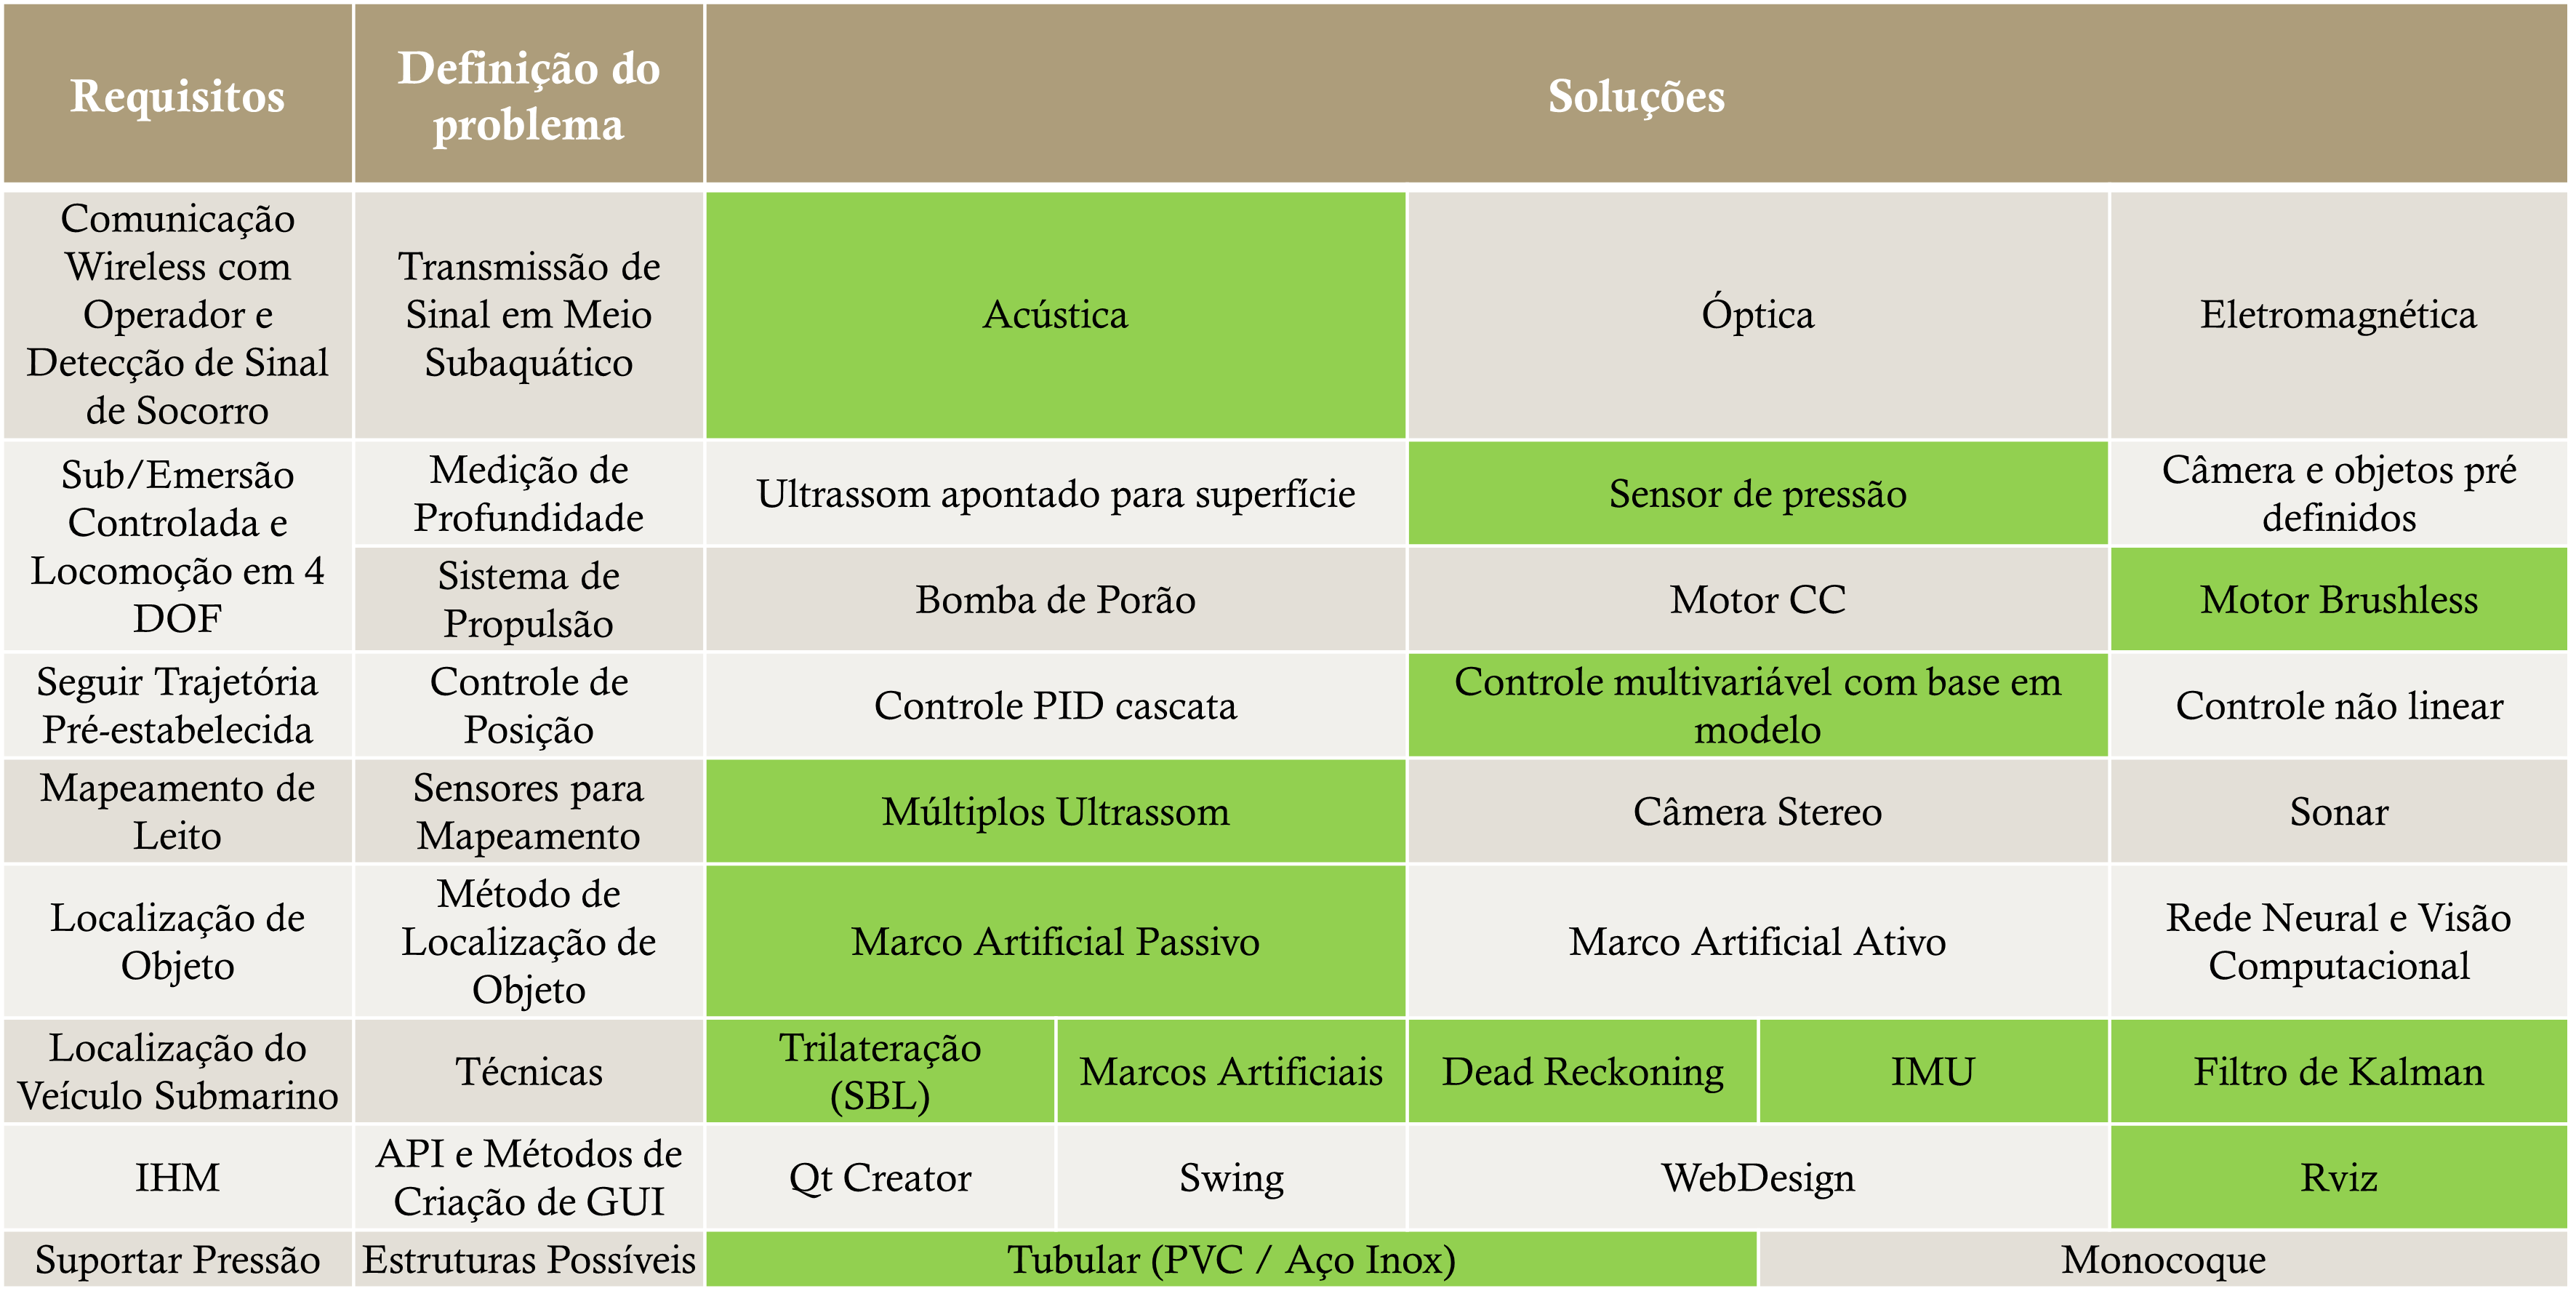
\includegraphics[width=1\linewidth]{images/Matriz-morfologica}\\
	\footnotesize Fonte: Autores
\end{table}

INSERIR ARGUMENTOS DA ESCOLHA DE CADA SENSOR DA MATRIZ MORFOLÓGICA.

\subsection{Projeto Conceitual}
\label{subsec:projeto-conceitual}


INSERIR EXPLICAÇÕES DO PROJETO CONCEITUAL, SIMILAR AO PRESENTE NA SUBSEÇÃO DE BRAINSTORMING.

\begin{figure}[h]
	\centering
	\caption{Conceito da solução após matriz morfológica}
	\label{fig:conceito-final}
	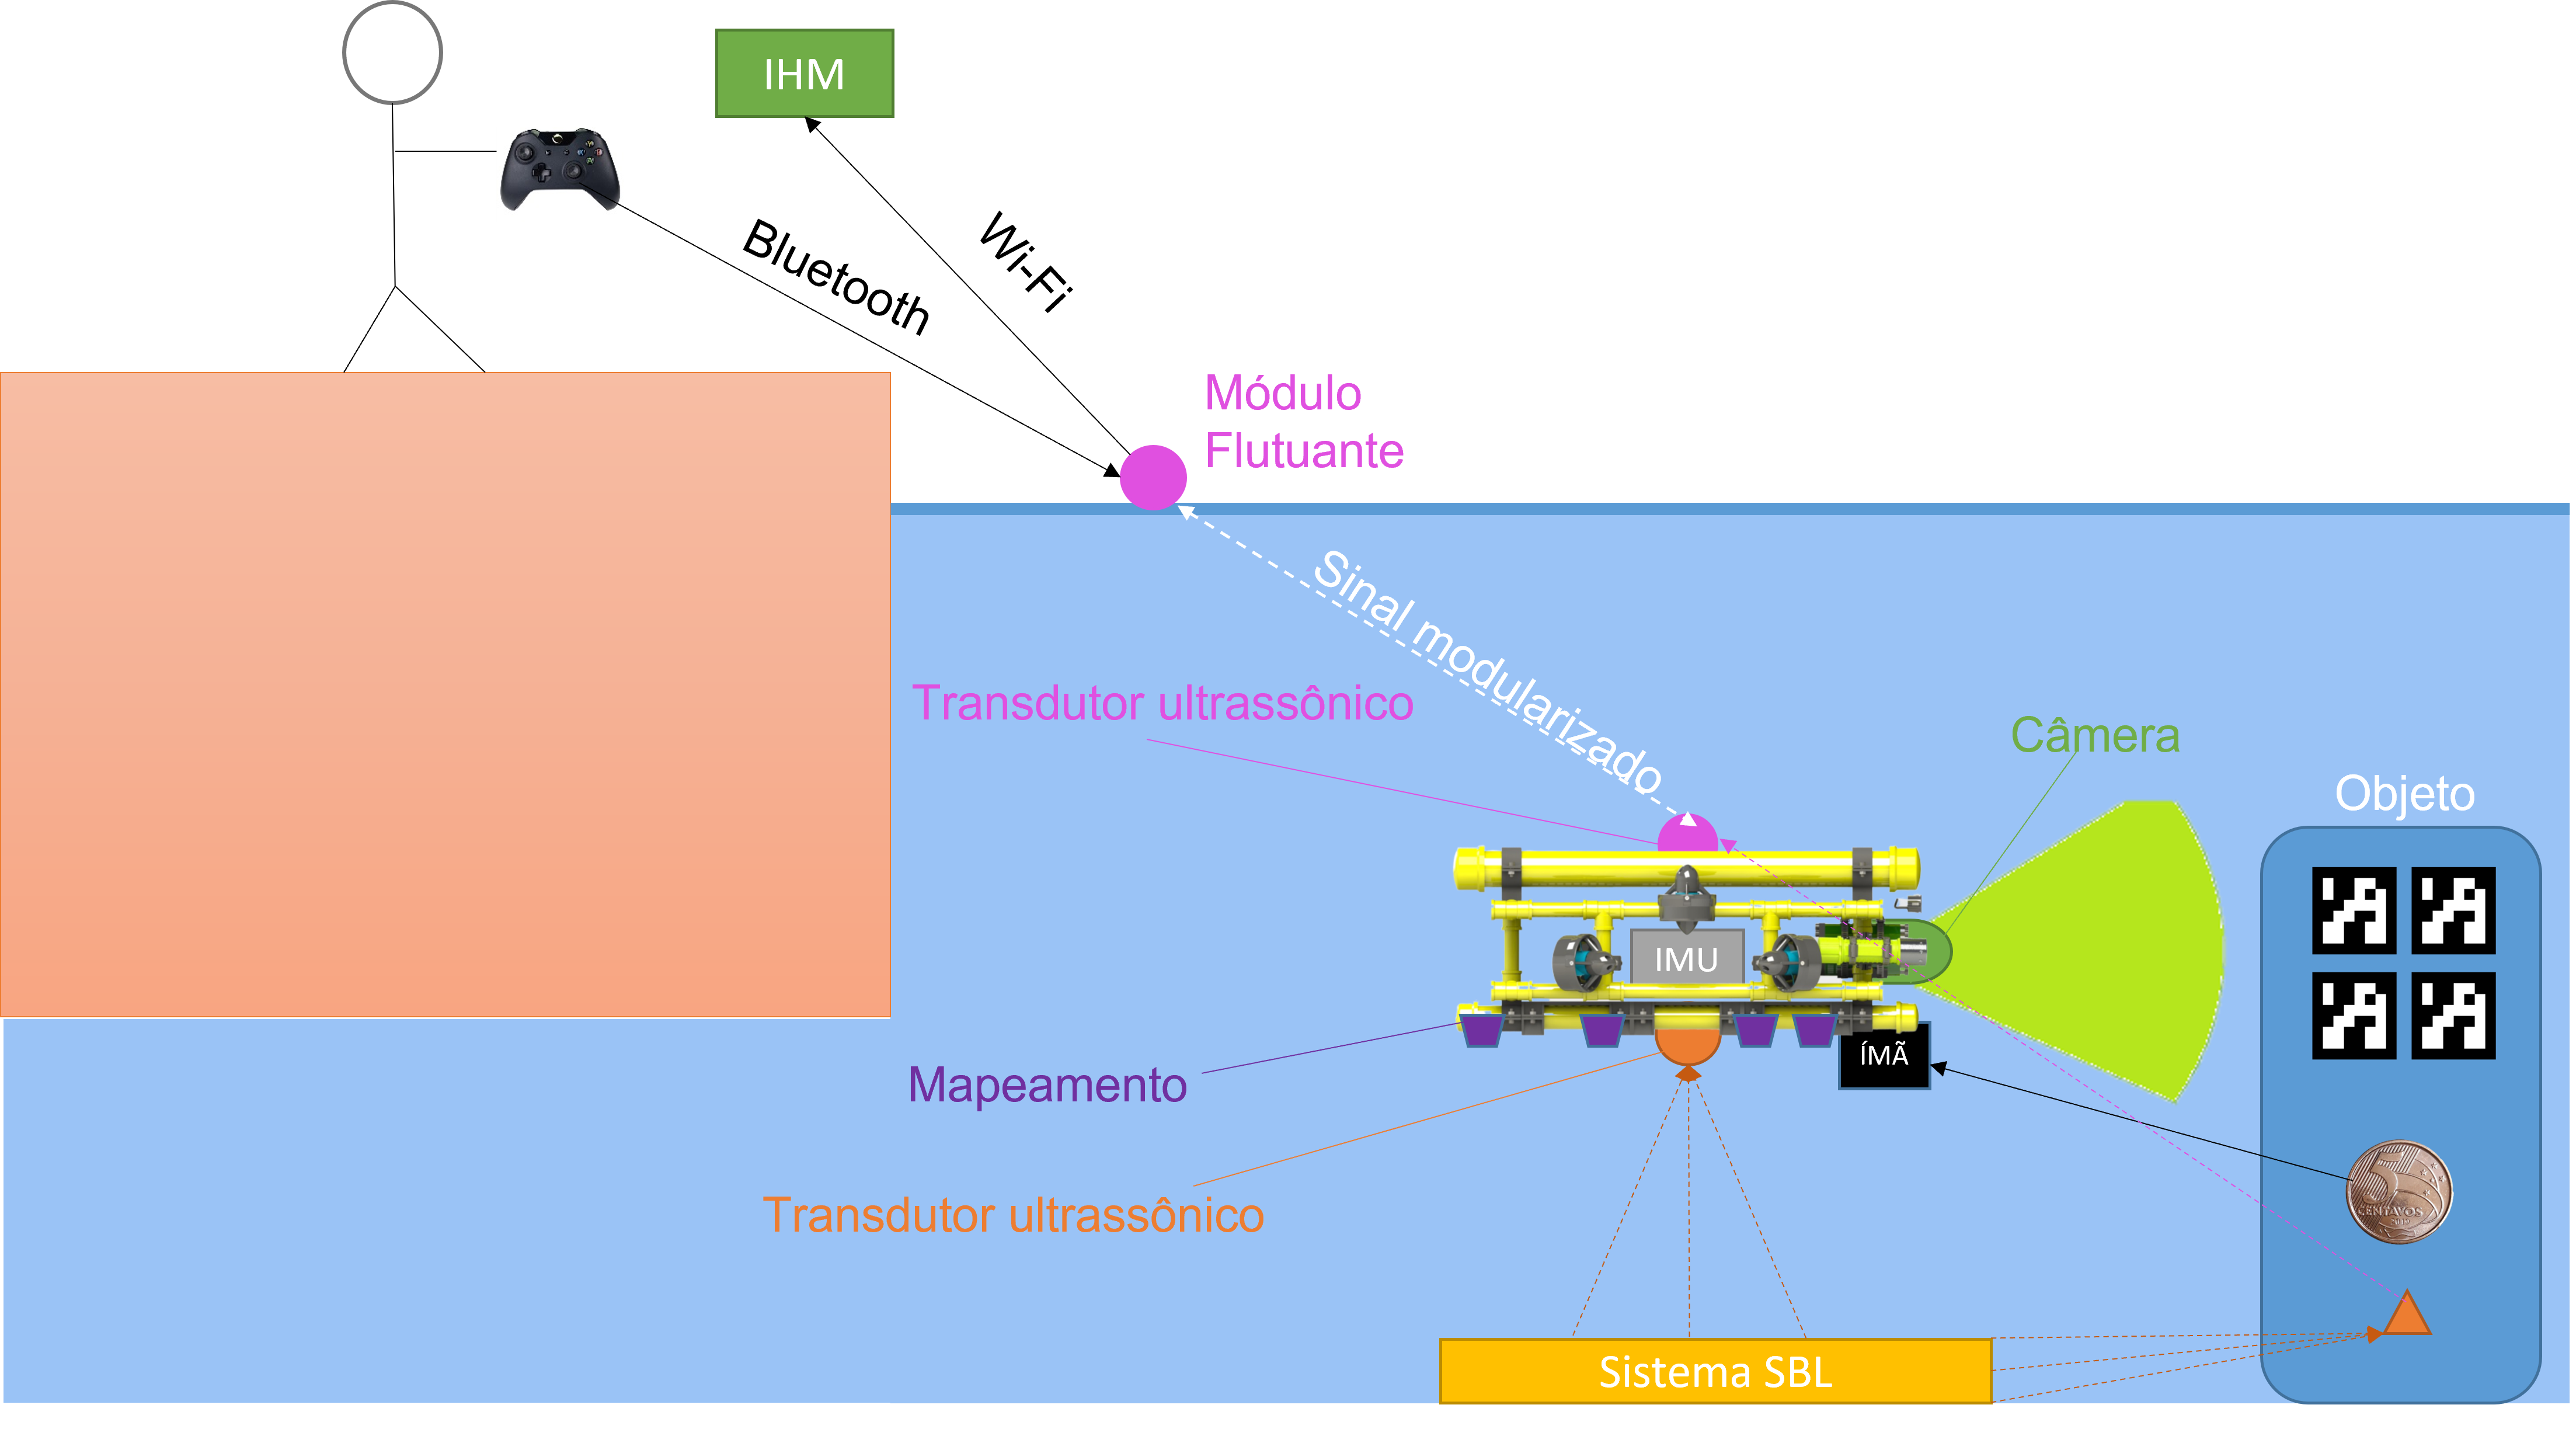
\includegraphics[width=1\linewidth]{images/conceito-final}\\
	\footnotesize Fonte: Autores
\end{figure}



